\chapter{Fungi}\label{fungi}

\href{https://en.wikipedia.org/wiki/Fungus}{Fungi} are uni- or
multicellular heterotrophic, eukaryotic organisms with external
digestion. Fungi include microorganisms such as yeasts and molds and
mushrooms. These organisms are classified as a kingdom, Fungi, which is
separate from the other eukaryotic life kingdoms of protists, plants and
animals. The English word fungus has been adopted from the Latin word
fungus (mushroom) which in turn is derived from the Greek word sphongos
meaning ``sponge''.

Fungi acquire their food by absorbing dissolved molecules, typically by
secreting digestive enzymes into their environment (a process referred
to as external digestion) unlike animals, which ingest food and digest
it internally in their digestive systems (a process referred to as
internal digestion). Fungi do not photosynthesize. Growth is their means
of mobility, except for spores (a few of which are flagellated), which
may travel through the air or water. Fungi are the principal decomposers
in ecological systems. These and other differences place fungi in a
single group of related organisms, named the Eumycota (true fungi or
Eumycetes), which share a common ancestor (form a monophyletic group),
an interpretation that is also strongly supported by molecular
phylogenetics. This fungal group is distinct from the structurally
similar myxomycetes (slime molds) and oomycetes (water molds). The
discipline of biology devoted to the study of fungi is known as mycology
(from the Greek mykes, mushroom). In the past, mycology was regarded as
a branch of botany, although it is now known fungi are genetically more
closely related to animals than to plants.

Abundant worldwide, most fungi are inconspicuous because of the small
size of their structures, and their cryptic lifestyles in soil or on
dead matter. Fungi include symbionts of plants, animals, or other fungi
and also parasites. They may become noticeable when fruiting, either as
mushrooms or as molds. Fungi perform an essential role in the
decomposition of organic matter and have fundamental roles in nutrient
cycling and exchange in the environment. They have long been used as a
direct source of human food, in the form of mushrooms and truffles; as a
leavening agent for bread; and in the fermentation of various food
products, such as wine, beer, and soy sauce. Since the 1940s, fungi have
been used for the production of antibiotics, and, more recently, various
enzymes produced by fungi are used industrially and in detergents. Fungi
are also used as biological pesticides to control weeds, plant diseases
and insect pests. Many species produce bioactive compounds called
mycotoxins that are toxic to animals including humans. The fruiting
structures of a few species contain psychotropic compounds and are
consumed recreationally or in traditional spiritual ceremonies. Fungi
can break down manufactured materials and buildings, and become
significant pathogens of humans and other animals. Losses of crops due
to fungal diseases (e.g., rice blast disease) or food spoilage can have
a large impact on human food supplies and local economies.

The fungus kingdom encompasses an enormous diversity of taxa with varied
ecologies, life cycle strategies, and morphologies ranging from
unicellular aquatic chytrids to large mushrooms. However, little is
known of the true biodiversity of Kingdom Fungi, which has been
estimated at 2.2 million to 3.8 million species, of which only 120,000
have been described. 8000 of them are detrimental to plants and 300 can
be pathogenic to humans. Ever since the pioneering 18th and 19th century
taxonomical works of Carl Linnaeus, Christian Hendrik Persoon, and Elias
Magnus Fries, fungi have been classified according to their morphology
(e.g., characteristics such as spore color or microscopic features) or
physiology. Advances in molecular genetics have opened the way for DNA
analysis to be incorporated into taxonomy, which has sometimes
challenged the historical groupings based on morphology and other
traits. Phylogenetic studies published in the last decade have helped
reshape the classification within Kingdom Fungi, which is divided into
one subkingdom, seven phyla, and ten subphyla.

\section{Microscopic Morphology}\label{microscopic-morphology}

Most fungi grow as hyphae, which are cylindrical, thread-like structures
2--10 µm in diameter and up to several centimeters in length. Hyphae
grow at their tips (apices); new hyphae are typically formed by
emergence of new tips along existing hyphae by a process called
branching, or occasionally growing hyphal tips fork, giving rise to two
parallel-growing hyphae. Hyphae also sometimes fuse when they come into
contact, a process called hyphal fusion (or anastamosis). These growth
processes lead to the development of a mycelium, an interconnected
network of hyphae. Hyphae can be either septate or coenocytic. Septate
hyphae are divided into compartments separated by cross walls (internal
cell walls, called septa, that are formed at right angles to the cell
wall giving the hypha its shape), with each compartment containing one
or more nuclei; coenocytic hyphae are not compartmentalized. Septa have
pores that allow cytoplasm, organelles, and sometimes nuclei to pass
through; an example is the dolipore septum in fungi of the phylum
Basidiomycota. Coenocytic hyphae are in essence multinucleate
supercells. Many species have developed specialized hyphal structures
for nutrient uptake from living hosts; examples include haustoria in
plant-parasitic species of most fungal phyla, and arbuscules of several
mycorrhizal fungi, which penetrate into the host cells to consume
nutrients. Although fungi are opisthokonts---a grouping of
evolutionarily related organisms broadly characterized by a single
posterior flagellum---all phyla except for the chytrids have lost their
posterior flagella. Fungi are unusual among the eukaryotes in having a
cell wall that, in addition to glucans (e.g., β-1,3-glucan) and other
typical components, also contains the biopolymer chitin.

\section{Macroscopic Morphology}\label{macroscopic-morphology}

Fungal mycelia can become visible to the naked eye, for example, on
various surfaces and substrates, such as damp walls and spoiled food,
where they are commonly called molds. Mycelia grown on solid agar media
in laboratory petri dishes are usually referred to as colonies. These
colonies can exhibit growth shapes and colors (due to spores or
pigmentation) that can be used as diagnostic features in the
identification of species or groups. Some individual fungal colonies can
reach extraordinary dimensions and ages as in the case of a clonal
colony of \emph{Armillaria solidipes}, which extends over an area of more than
900 ha (3.5 square miles), with an estimated age of nearly 9,000 years.
The apothecium---a specialized structure important in sexual
reproduction in the ascomycetes---is a cup-shaped fruit body that is
often macroscopic and holds the hymenium, a layer of tissue containing
the spore-bearing cells. The fruit bodies of the basidiomycetes
(basidiocarps) and some ascomycetes (ascocarps) can sometimes grow very
large, and many are well known as mushrooms.

\section{Reproduction}\label{reproduction}

Fungal reproduction is complex, reflecting the differences in lifestyles
and genetic makeup within this diverse kingdom of organisms. It is
estimated that a third of all fungi reproduce using more than one method
of propagation. Environmental conditions trigger genetically determined
developmental states that lead to the creation of specialized structures
for sexual or asexual reproduction. These structures aid reproduction by
efficiently dispersing spores or spore-containing propagules.

Asexual reproduction occurs via vegetative spores (conidia) or through
mycelial fragmentation. Mycelial fragmentation occurs when a fungal
mycelium separates into pieces, and each component grows into a separate
mycelium. Mycelial fragmentation and vegetative spores maintain clonal
populations adapted to a specific niche, and allow more rapid dispersal
than sexual reproduction. The ``Fungi imperfecti'' (fungi lacking the
perfect or sexual stage) or Deuteromycota comprise all the species that
lack an observable sexual cycle. Deuteromycota is not an accepted
taxonomic clade, and is now taken to mean simply fungi that lack a known
sexual stage.

\section{\texorpdfstring{\emph{Aspergillus}}{Aspergillus}}\label{aspergillus}

\href{https://en.wikipedia.org/wiki/Aspergillus}{\emph{Aspergillus}} is
a genus consisting of a few hundred species of mold found in various
climates worldwide. \emph{Aspergillus} was first catalogued in 1729 by the
Italian priest and biologist Pier Antonio Micheli. Viewing the fungi
under a microscope, Micheli was reminded of the shape of an aspergillum
(holy water sprinkler), from Latin spargere (to sprinkle), and named the
genus accordingly. Aspergillum is an asexual spore-forming structure
common to all \emph{Aspergillus} species; around one-third of species are also
known to have a sexual stage.

\section{\texorpdfstring{\emph{Penicillium}}{Penicillium}}\label{penicillium}

\href{https://en.wikipedia.org/wiki/Penicillium}{\emph{Penicillium}}
ascomycetous fungi are of major importance in the natural environment as
well as food and drug production. Some members of the genus produce
penicillin, a molecule that is used as an antibiotic, which kills or
stops the growth of certain kinds of bacteria. Other species are used in
cheesemaking. The genus was first described in the scientific literature
by Johann Heinrich Friedrich Link in his 1809 work Observationes in
ordines plantarum naturales, writing ``Penicillium. Thallus e floccis
caespitosis septatis simplicibus aut ramosis fertilibus erectis apice
penicillatis'', where penicillatis referred to ``pencil-like''
(referring to a Camel's hair pencil brush).

\section{\texorpdfstring{\emph{Rhizopus
stolonifer}}{Rhizopus stolonifer}}\label{rhizopus-stolonifer}

\href{https://en.wikipedia.org/wiki/Rhizopus_stolonifer}{\emph{Rhizopus
stolonifer}} is commonly known as black bread mold. It is a member of
Zygomycota and considered the most important species in the genus
\emph{Rhizopus}. It is one of the most common fungi in the world and has a
global distribution although it is most commonly found in tropical and
subtropical regions. It is a common agent of decomposition of stored
foods. Like other members of the genus \emph{Rhizopus}, \emph{R. stolonifer} grows
rapidly, mostly in indoor environments.

\section{Yeast}\label{yeast}

\href{https://en.wikipedia.org/wiki/Yeast}{Yeasts} are single-celled
fungi. The first yeast originated hundreds of millions of years ago, and
1,500 species are currently identified. They are estimated to constitute
1\% of all described fungal species. Yeasts are unicellular organisms
which evolved from multicellular ancestors, with some species having the
ability to develop multicellular characteristics by forming strings of
connected budding cells known as pseudohyphae or false hyphae. Yeast
sizes vary greatly, depending on species and environment, typically
measuring 3--4 µm in diameter, although some yeasts can grow to 40 µm in
size. Most yeasts reproduce asexually by mitosis, and many do so by the
asymmetric division process known as budding.

Yeasts, with their single-celled growth habit, can be contrasted with
molds, which grow hyphae. Fungal species that can take both forms
(depending on temperature or other conditions) are called dimorphic
fungi (``dimorphic'' means ``having two forms'').

By fermentation, the yeast species \emph{Saccharomyces cerevisiae}
converts carbohydrates to carbon dioxide and alcohols -- for thousands
of years the carbon dioxide has been used in baking and the alcohol in
alcoholic beverages. It is also a centrally important model organism in
modern cell biology research, and is one of the most thoroughly
researched eukaryotic microorganisms. Researchers have used it to gather
information about the biology of the eukaryotic cell and ultimately
human biology. Other species of yeasts, such as \emph{Candida albicans},
are opportunistic pathogens and can cause infections in humans.

Yeasts do not form a single taxonomic or phylogenetic grouping. The term
``yeast'' is often taken as a synonym for \emph{Saccharomyces
cerevisiae} (baker's or brewer's yeast) but the phylogenetic diversity
of yeasts is shown by their placement in two separate phyla: the
Ascomycota and the Basidiomycota. The budding yeasts (``true yeasts'')
are classified in the order Saccharomycetales, within the phylum
Ascomycota.

\section{View Prepared Slides of Fungi Lacking Sexual
Stages}\label{view-the-prepared-slides-of-fungi-lacking-sexual-stages}

\begin{enumerate}
\def\labelenumi{\arabic{enumi}.}
\tightlist
\item
  \emph{Aspergillus} conidiophores (Figure \ref{fig:aspergillus})

  \begin{itemize}
  \tightlist
  \item
    Locate: conidiophores and conidiospores
  \end{itemize}
\item
  \emph{Penicillium} (Figure \ref{fig:penicillium})

  \begin{itemize}
  \tightlist
  \item
    Locate: conidiophores and conidiospores (asexual spores)
  \end{itemize}
\item
  \emph{Penicillium} on orange peel (Figure \ref{fig:orange})
\end{enumerate}



\begin{figure}

{\centering \includegraphics[width=0.7\linewidth]{./figures/fungi/aspergillus}

}

\caption{\emph{Aspergillus} conidiophores.}\label{fig:aspergillus}
\end{figure}



\begin{figure}

{\centering \includegraphics[width=0.7\linewidth]{./figures/fungi/penicillium}

}

\caption{\emph{Penicillium} conidiophores.}\label{fig:penicillium}
\end{figure}



\begin{figure}

{\centering \includegraphics[width=0.7\linewidth]{./figures/fungi/penicillium_orange}

}

\caption{\emph{Penicillium} growing on orange peel.}\label{fig:orange}
\end{figure}

Sexual reproduction with meiosis has been directly observed in all
fungal phyla except Glomeromycota (genetic analysis suggests meiosis in
Glomeromycota as well). It differs in many aspects from sexual
reproduction in animals or plants. Differences also exist between fungal
groups and can be used to discriminate species by morphological
differences in sexual structures and reproductive strategies. The major
fungal groupings have initially been delineated based on the morphology
of their sexual structures and spores; for example, the spore-containing
structures, asci (sacs) and basidia (clubs), can be used in the
identification of ascomycetes (sac fungi) and basidiomycetes (club
fungi), respectively. Some species may allow mating only between
individuals of opposite mating type, whereas others can mate and
sexually reproduce with any other individual or itself. Species of the
former mating system are called heterothallic, and of the latter
homothallic.

Most fungi have both a haploid and a diploid stage in their life cycles.
In sexually reproducing fungi, compatible individuals may combine by
fusing their hyphae together into an interconnected network; this
process, anastomosis, is required for the initiation of the sexual
cycle. Many ascomycetes and basidiomycetes go through a dikaryotic
stage, in which the nuclei inherited from the two parents do not combine
immediately after cell fusion, but remain separate in the hyphal cells.

In ascomycetes, dikaryotic hyphae of the hymenium (the spore-bearing
tissue layer) form a characteristic hook at the hyphal septum. During
cell division, formation of the hook ensures proper distribution of the
newly divided nuclei into the apical and basal hyphal compartments. An
ascus (plural asci) is then formed, in which karyogamy (nuclear fusion)
occurs. Asci are embedded in an ascocarp, or fruiting body. Karyogamy in
the asci is followed immediately by meiosis and the production of
ascospores. After dispersal, the ascospores may germinate and form a new
haploid mycelium.

\section{View Prepared Slides of
Ascomycetes}\label{view-the-prepared-slides-ascomycetes}

\begin{enumerate}
\def\labelenumi{\arabic{enumi}.}
\tightlist
\item
  \href{https://en.wikipedia.org/wiki/Peziza}{\emph{Peziza}}
  (Figure \ref{fig:peziza}) apothecium

  \begin{itemize}
  \tightlist
  \item
    Locate: Hymenium layer, ascus with 8 ascospores, and infertile
    hyphae
  \end{itemize}
\item
  Yeast (Figure \ref{fig:yeast})
\end{enumerate}



\begin{figure}

{\centering 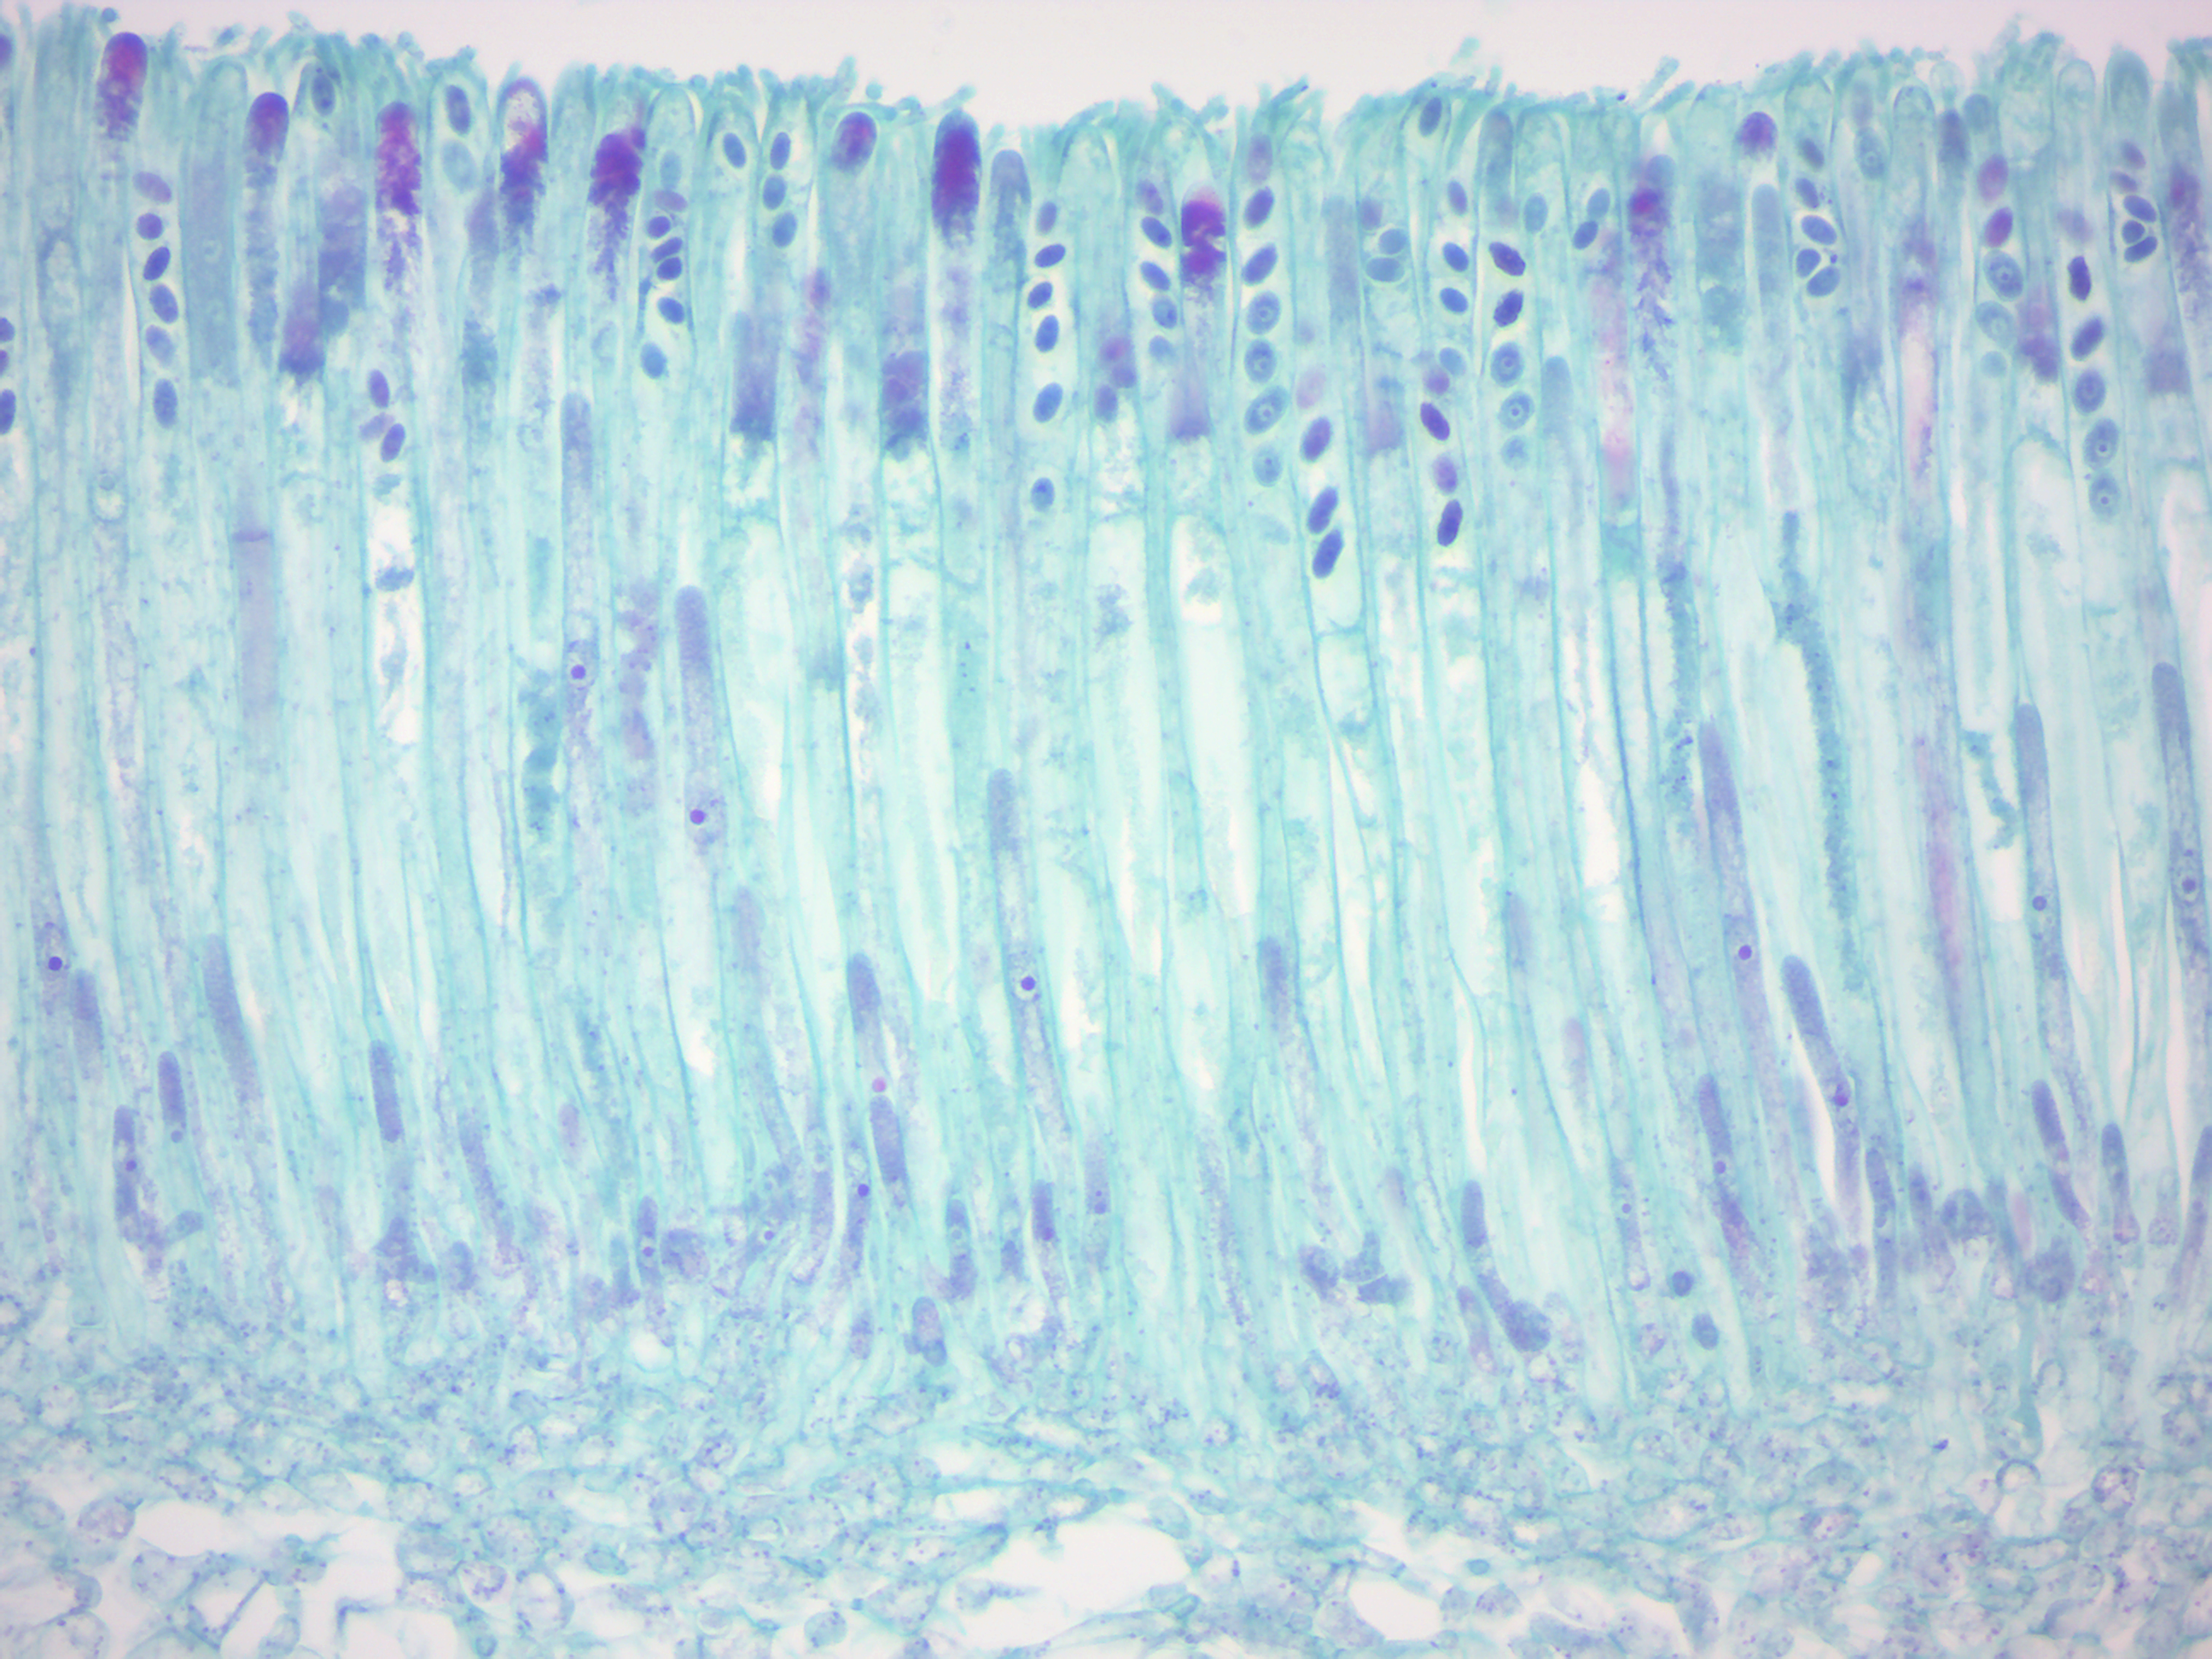
\includegraphics[width=0.7\linewidth]{./figures/fungi/peziza_apothecium}

}

\caption{\emph{Peziza} apothecium.}\label{fig:peziza}
\end{figure}

\begin{figure}

{\centering 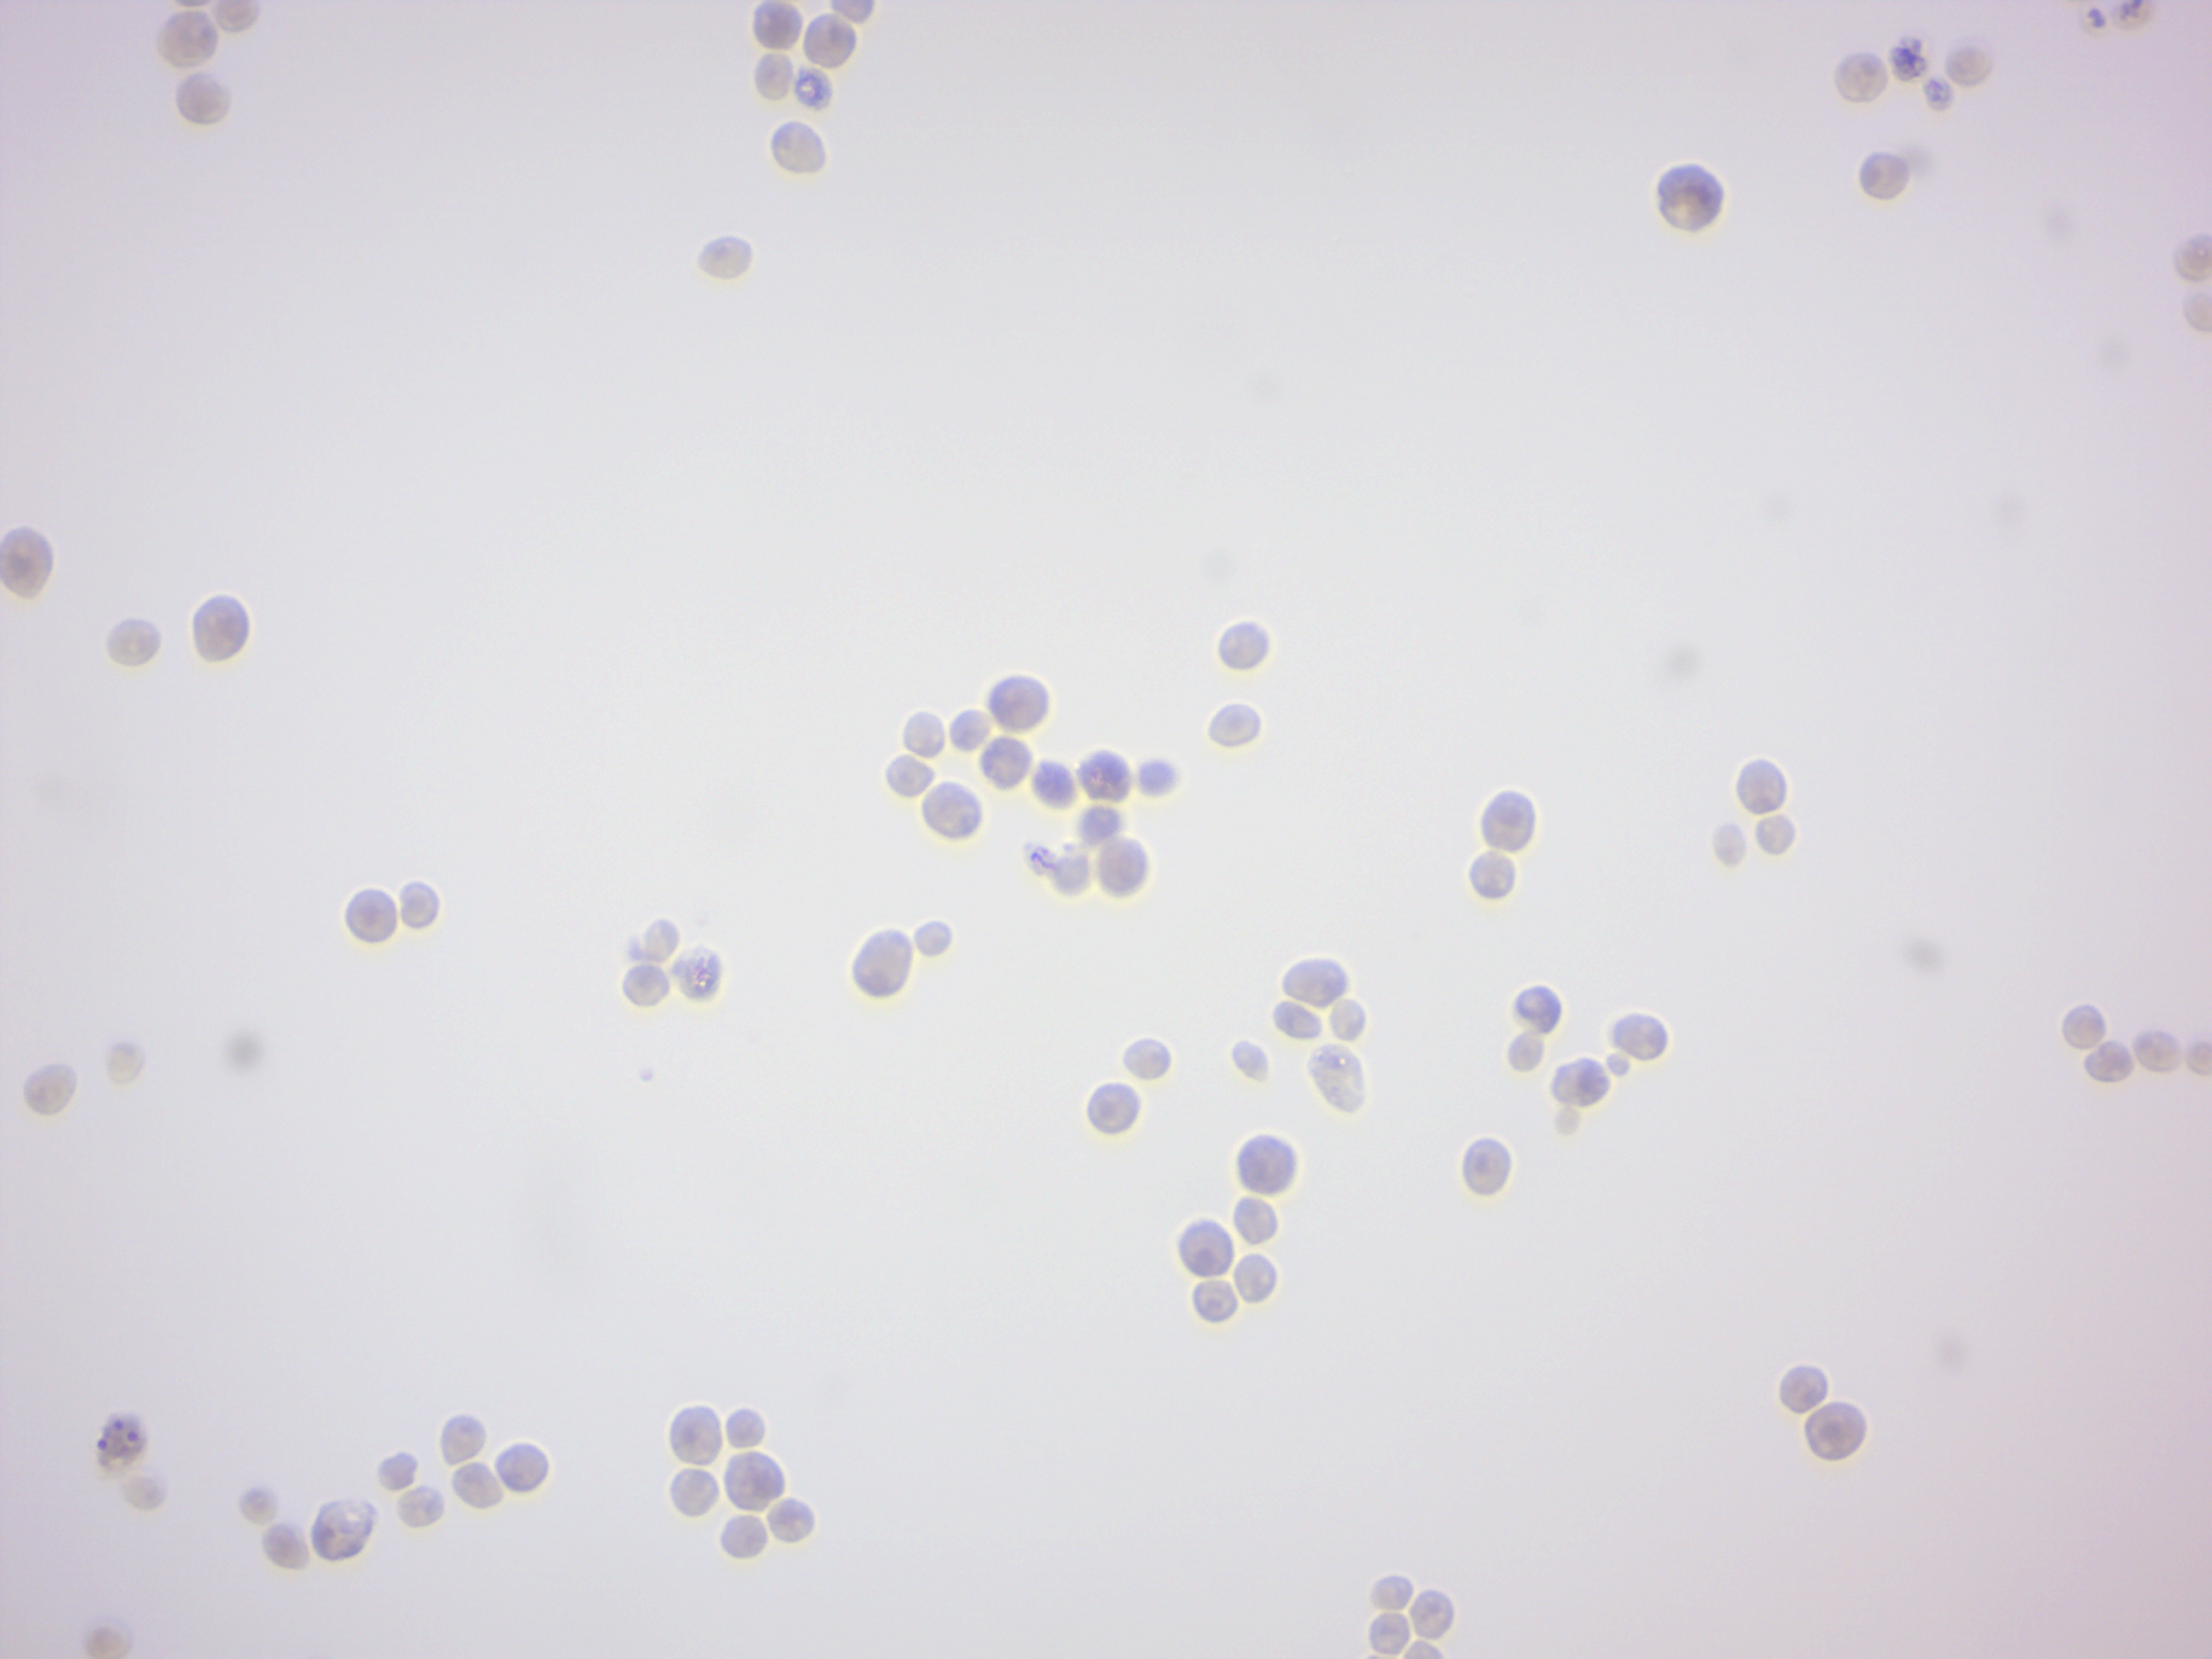
\includegraphics[width=0.7\linewidth]{./figures/fungi/yeast}

}

\caption{Yeast.}\label{fig:yeast}
\end{figure}

\section{View Prepared Slides of
Basidiomycetes}\label{view-the-prepared-slides-of-basidiomycetes}

Sexual reproduction in basidiomycetes is similar to that of the
ascomycetes. Compatible haploid hyphae fuse to produce a dikaryotic
mycelium. However, the dikaryotic phase is more extensive in the
basidiomycetes, often also present in the vegetatively growing mycelium.
A specialized anatomical structure, called a clamp connection, is formed
at each hyphal septum. As with the structurally similar hook in the
ascomycetes, the clamp connection in the basidiomycetes is required for
controlled transfer of nuclei during cell division, to maintain the
dikaryotic stage with two genetically different nuclei in each hyphal
compartment. A basidiocarp is formed in which club-like structures known
as basidia generate haploid basidiospores after karyogamy and meiosis.
The most commonly known basidiocarps are mushrooms, but they may also
take other forms.

\begin{enumerate}
\def\labelenumi{\arabic{enumi}.}
\tightlist
\item
  \href{https://en.wikipedia.org/wiki/Coprinus}{\emph{Coprinus}} (Figure
  \ref{fig:basidia})

  \begin{itemize}
  \tightlist
  \item
    Locate: gills, basidium with 4 basidiospores, hyphae
  \end{itemize}
\end{enumerate}

\begin{figure}

{\centering \includegraphics[width=0.7\linewidth]{./figures/fungi/basidia}

}

\caption{\emph{Coprinus} basidia with spores.}\label{fig:basidia}
\end{figure}

\section{View Prepared Slides
Glomeromycetes}\label{view-the-prepared-slides-glomeromycetes}

In glomeromycetes (formerly zygomycetes), haploid hyphae of two
individuals fuse, forming a gametangium, a specialized cell structure
that becomes a fertile gamete-producing cell. The gametangium develops
into a zygospore, a thick-walled spore formed by the union of gametes.
When the zygospore germinates, it undergoes meiosis, generating new
haploid hyphae, which may then form asexual sporangiospores. These
sporangiospores allow the fungus to rapidly disperse and germinate into
new genetically identical haploid fungal mycelia.

\begin{enumerate}
\def\labelenumi{\arabic{enumi}.}
\tightlist
\item
  \emph{Rhizopus} sporangia (Figure \ref{fig:rhizopussporangia})

  \begin{itemize}
  \tightlist
  \item
    Locate: sporangium with spores, sporangiophore, and rhizoid and
    stolon, if possible
  \end{itemize}
\item
  \emph{Rhizopus} conjugation (Figure \ref{fig:rhizopusconjugation})

  \begin{itemize}
  \tightlist
  \item
    Locate: gametangia (isogametes), zygospores, and various kinds of
    hyphae
  \end{itemize}
\item
  \emph{Rhizopus} combination (sporangia and zygotes)

  \begin{itemize}
  \tightlist
  \item
    Locate: sporangium with spores, zygospores, gametangia, and hyphae
  \end{itemize}
\end{enumerate}



\begin{figure}

{\centering \includegraphics[width=0.7\linewidth]{./figures/fungi/rhizopus_sporangia}

}

\caption{\emph{Rhizopus} sporangia.}\label{fig:rhizopussporangia}
\end{figure}



\begin{figure}

{\centering 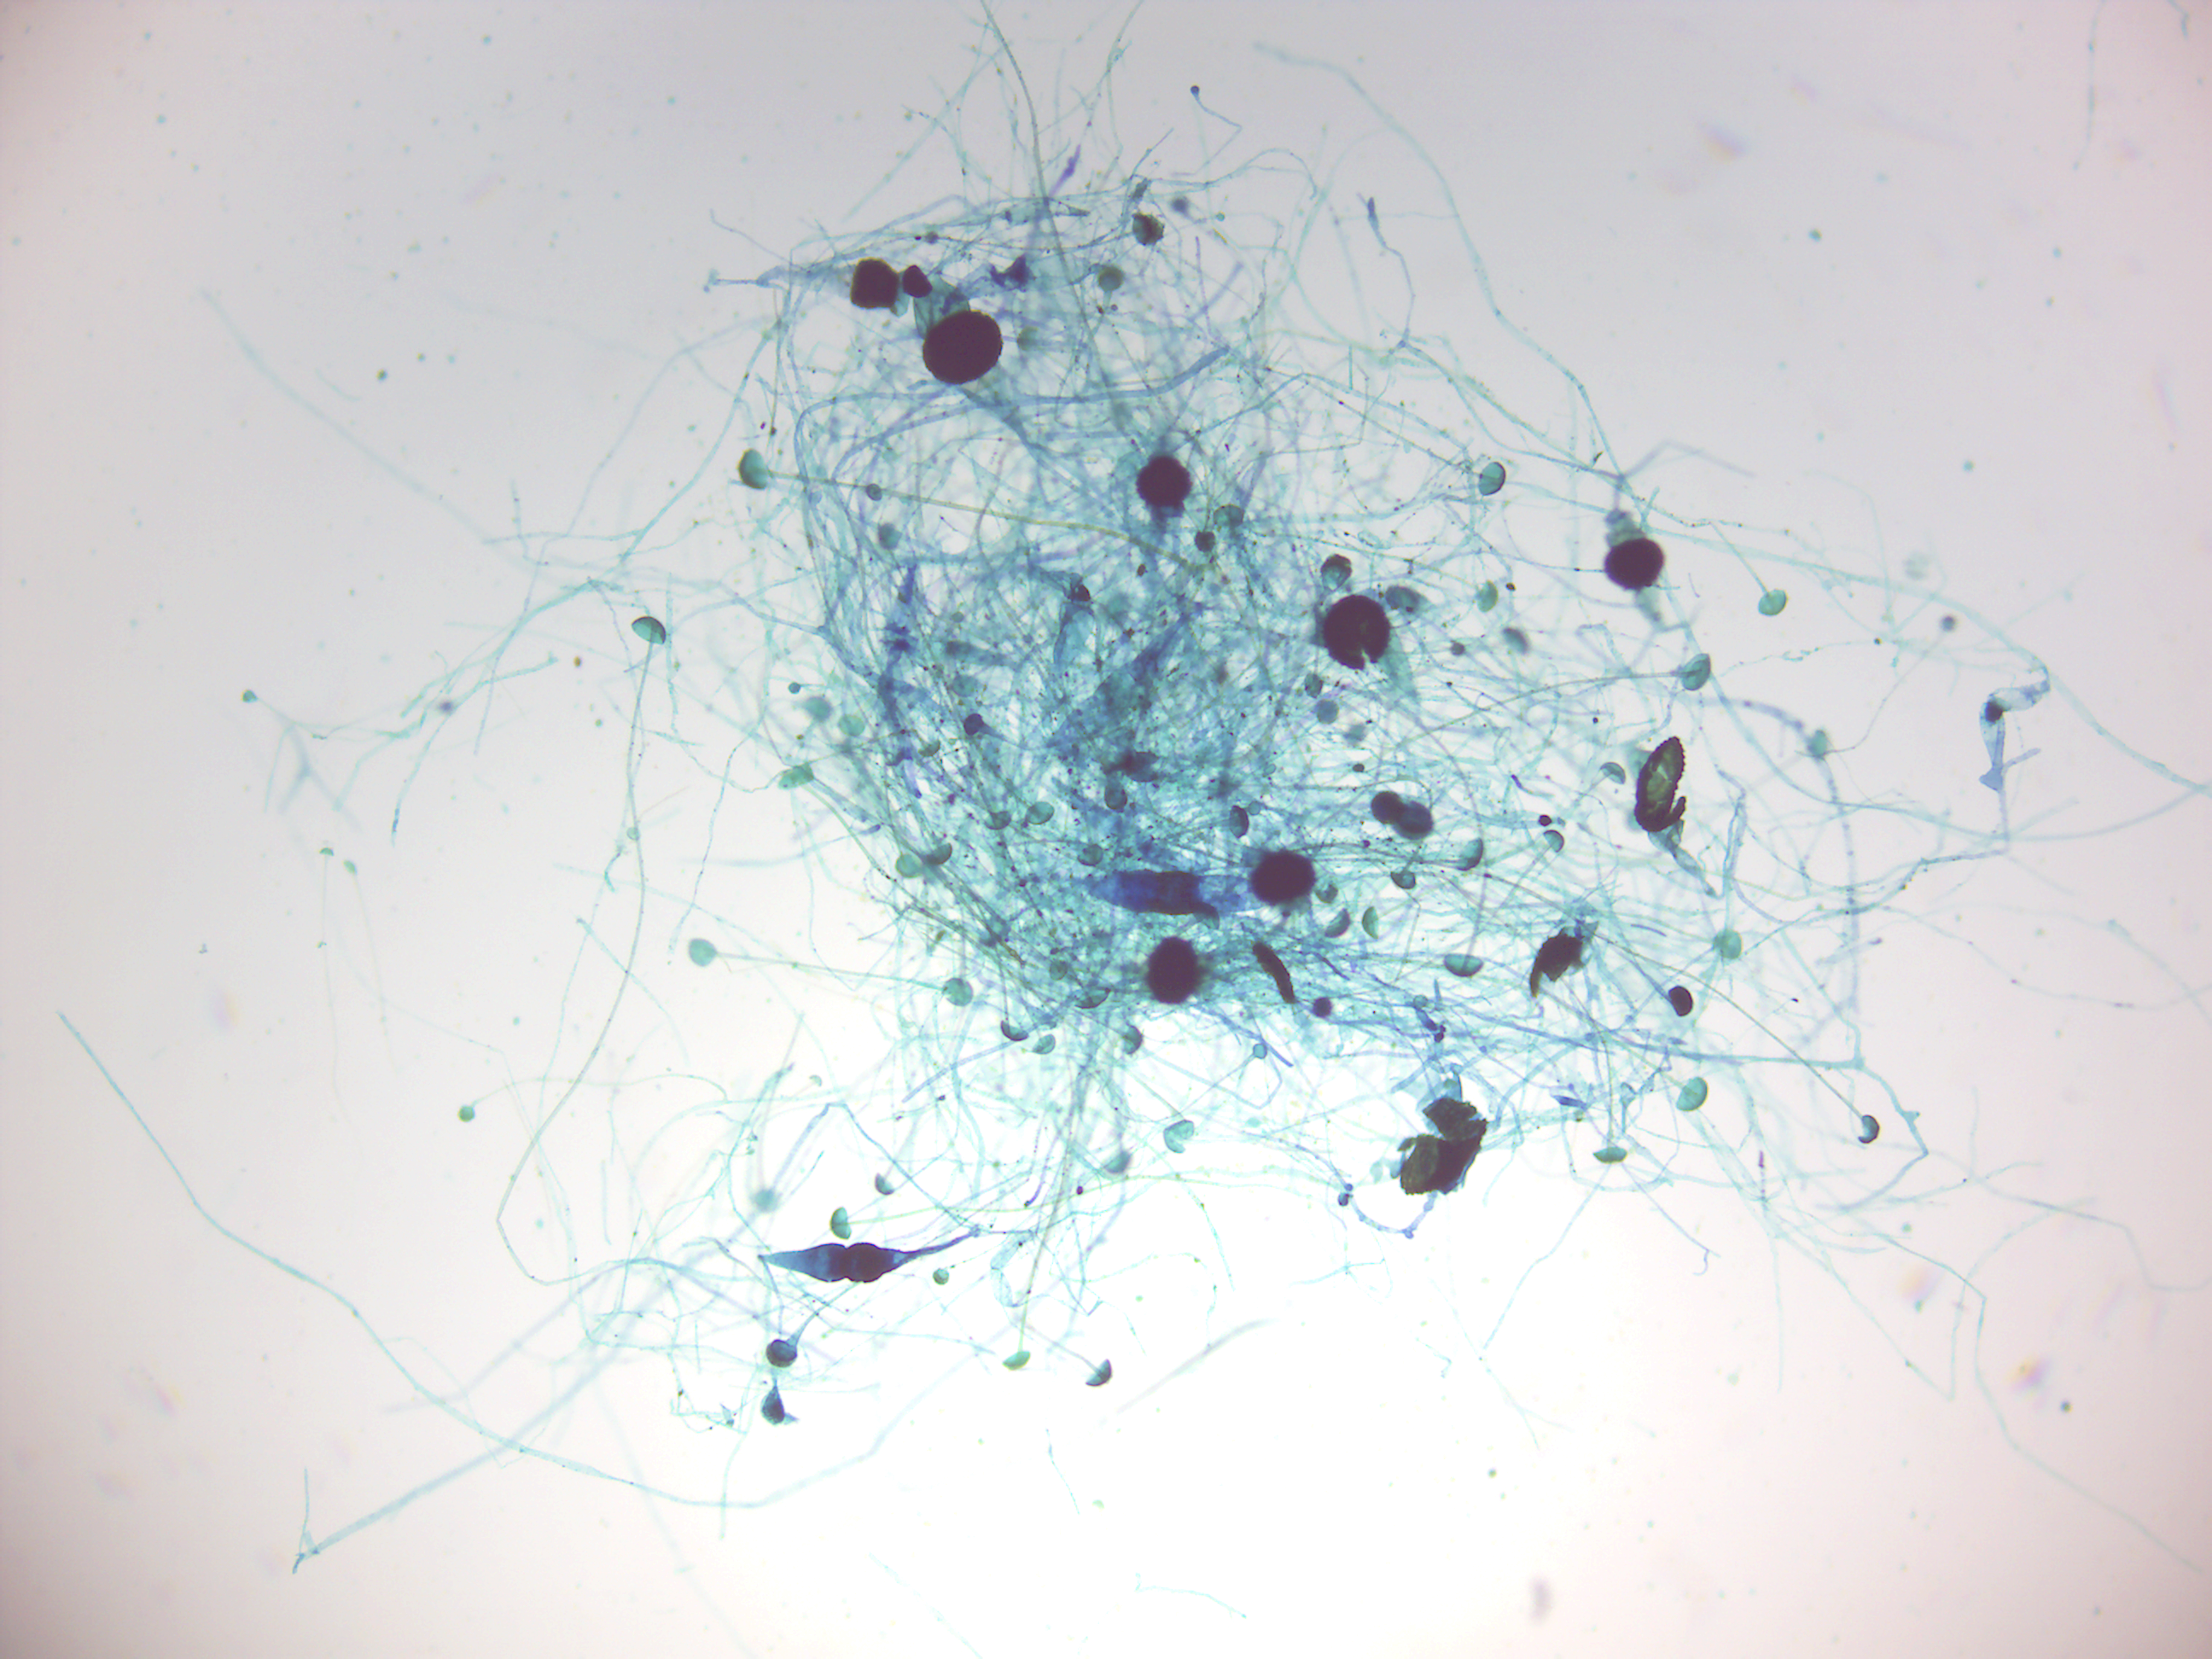
\includegraphics[width=0.7\linewidth]{./figures/fungi/rhizopus_conjugation}

}

\caption{\emph{Rhizopus} conjugation.}\label{fig:rhizopusconjugation}
\end{figure}

\section{Lichen}\label{lichen}

A \href{https://en.wikipedia.org/wiki/Lichen}{lichen} (Figure
\ref{fig:lichens}) is a composite organism that arises from algae or
cyanobacteria living among filaments of multiple fungi in a symbiotic
relationship. The combined lichen has properties different from those of
its component organisms. Lichens come in many colors, sizes, and forms.
The properties are sometimes plant-like, but lichens are not plants.
Lichens may have tiny, leafless branches (fruticose), flat leaf-like
structures (foliose), flakes that lie on the surface like peeling paint
(crustose), or other growth forms. Lichens occur from sea level to high
alpine elevations, in many environmental conditions, and can grow on
almost any surface. Lichens are abundant growing on bark, leaves,
mosses, on other lichens, and hanging from branches ``living on thin
air'' (epiphytes) in rain forests and in temperate woodland. They grow
on rock, walls, gravestones, roofs, exposed soil surfaces, and in the
soil as part of a biological soil crust. Different kinds of lichens have
adapted to survive in some of the most extreme environments on Earth:
arctic tundra, hot dry deserts, rocky coasts, and toxic slag heaps. They
can even live inside solid rock, growing between the grains. It is
estimated that 6\% of Earth's land surface is covered by lichen. There
are about 20,000 known species of lichens. Lichens may be long-lived,
with some considered to be among the oldest living things. They are
among the first living things to grow on fresh rock exposed after an
event such as a landslide. The long life-span and slow and regular
growth rate of some lichens can be used to date events.



\begin{figure}

{\centering 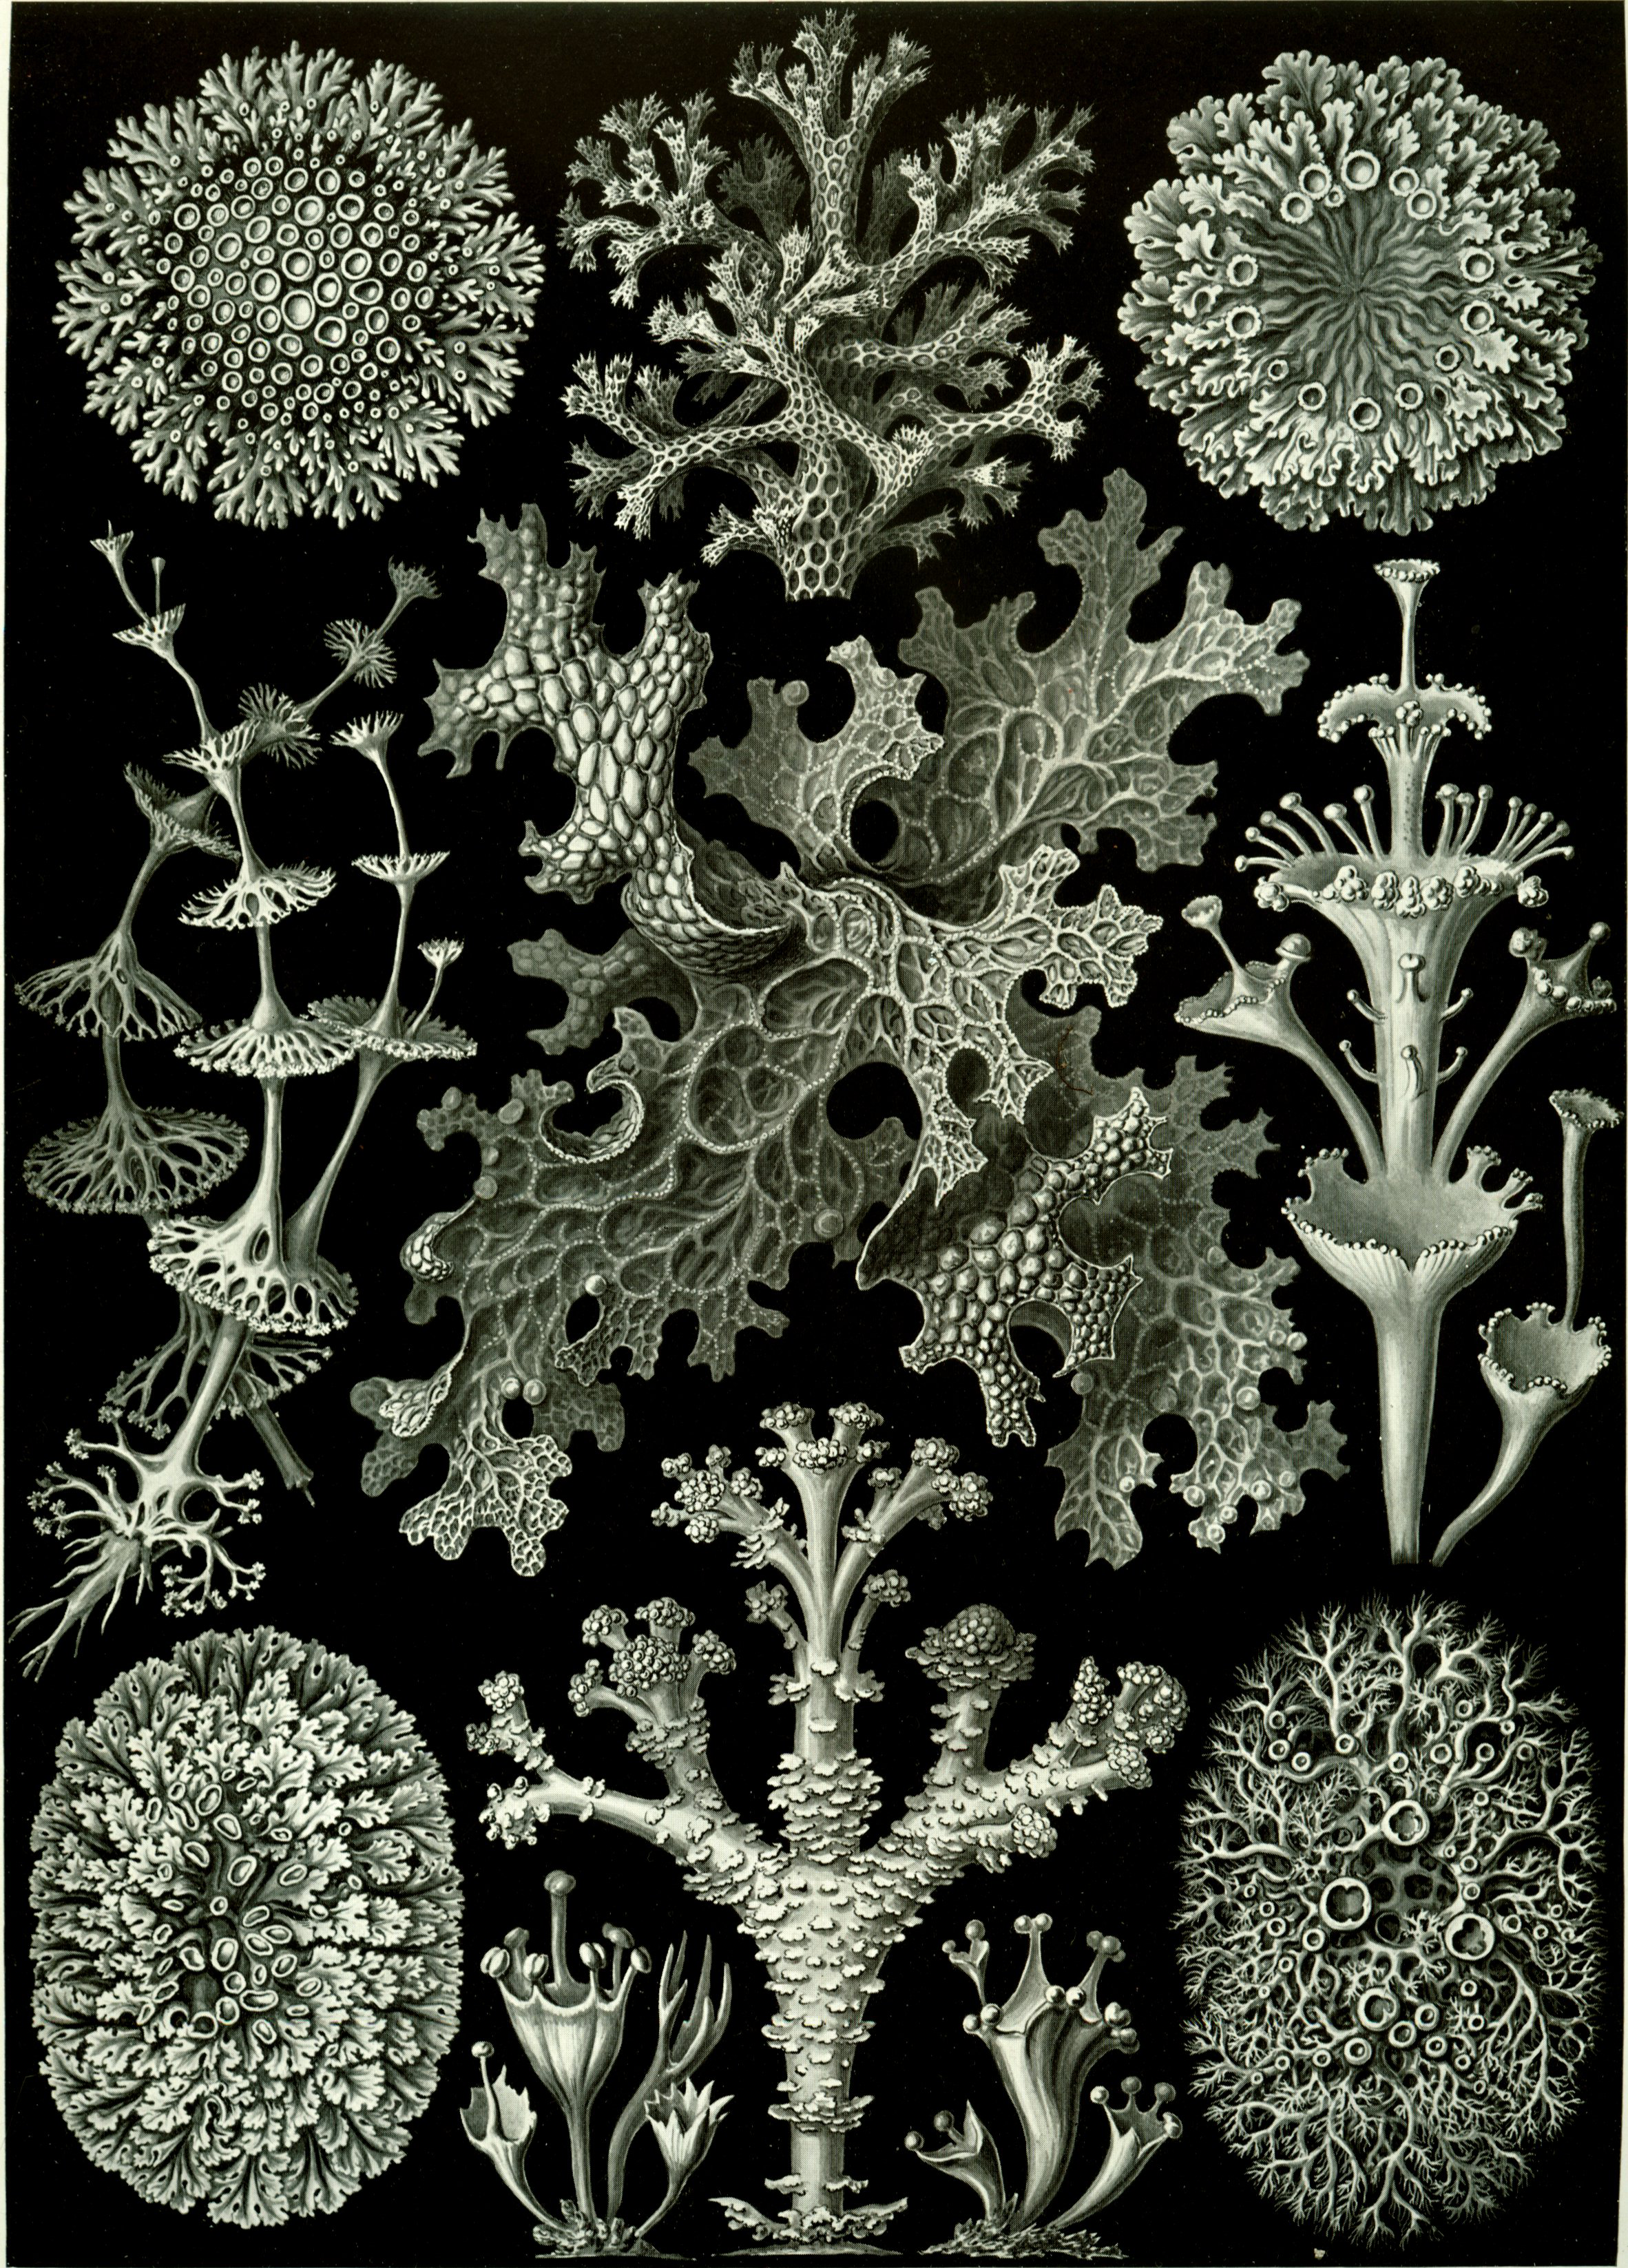
\includegraphics[width=0.7\linewidth]{./figures/fungi/Haeckel_Lichenes}

}

\caption{\href{https://commons.wikimedia.org/wiki/File:Haeckel_Lichenes.jpg}{Lichens}
from Ernst Haeckel's
\href{https://en.wikipedia.org/wiki/Kunstformen_der_Natur}{Kunstformen
der Natur}, 1904.}\label{fig:lichens}
\end{figure}

\section{View Prepared Slides of
Lichens}\label{view-the-prepared-slides-of-lichens}

\begin{enumerate}
\def\labelenumi{\arabic{enumi}.}
\tightlist
\item
  Foliose lichen thallus and apothecia (Figure \ref{fig:lichen})

  \begin{itemize}
  \tightlist
  \item
    Locate: fungal hyphae, and algal cells inside
  \end{itemize}
\end{enumerate}

\begin{figure}

{\centering \includegraphics[width=0.7\linewidth]{./figures/fungi/foliose_lichen}

}

\caption{Foliose lichen thallus and apothecia.}\label{fig:lichen}
\end{figure}

\section{View Living Organisms}\label{view-living-organisms}

\begin{enumerate}
\def\labelenumi{\arabic{enumi}.}
\tightlist
\item
  Yeast
\item
  \emph{Rhizopus stolonifer} plate
\item
  \emph{Aspergillus} plate
\item
  \emph{Penicillium} plate
\end{enumerate}

\section{Review Questions}\label{review-questions}

\begin{enumerate}
\def\labelenumi{\arabic{enumi}.}
\tightlist
\item
  What are fungi?
\item
  How do fungi get their nutrients?
\item
  What are yeasts?
\item
  What are lichen?
\item
  What is the name of the spore containing structure in sac fungi?
\item
  In club fungi, spores are attached to \underline{\phantom{answer}}.
\item
  What is a zygospore?
\item
  What are conidiophores?
\end{enumerate}
